
\chapter{Einleitung}
Einen Forschungsschwerpunkt am \ac{IPA} der \ac{FhG} bildet das Thema 
Servicerobotik. Die 1996 vom \ac{IPA} verfasste Definition für Serviceroboter 
ist auch heute noch gültig:

\begin{quote}"'Ein Serviceroboter ist 
eine frei programmierbare Bewegungseinrichtung, die teil- oder vollautomatisch 
Dienstleistungen verrichtet. Dienstleistungen sind dabei Tätigkeiten, die nicht 
der direkten industriellen Erzeugung von Sachgütern, sondern der Verrichtung von 
Leistungen für Menschen und Einrichtungen dienen."'\cite{Schraft1996}\end{quote} 

Das Ziel der Servicerobotikforschung ist es, den Menschen bei alltäglichen Aufgaben zu 
unterstützen. Weit verbreitete Beispiele für den Einsatz von Servicerobotern im 
häuslichen Bereich sind autonome Staubsauger oder Rasenmäher. Der häusliche 
Einsatz von Servicerobotern ist ein wichtiges Ziel der heutigen Forschung. 
Zusätzlich zu den oben angesprochenen einfachen Bauformen für Serviceroboter 
gibt es Roboter für komplexere Aufgaben, die aber noch nicht verbreitet oder 
erhältlich sind. Beispiele hierfür sind Tankroboter, die dem Kunden beim Tanken 
die "'Schmutzarbeit"'\nocite{tankpitstop} abnehmen oder persönliche Assistenten, 
wie dem PR2 von Willow Garage\footnote{Willow Garage ist ein Kalifornisches 
Unternehmen, das die Entwicklung ziviler Roboter durch Hardware und Open-Source
Software beschleunigen will.} oder der \cob des \ac{IPA}. Die beiden letztgenannten 
wurden als vielseitige Assistenten entwickelt, die in verschiedenen 
Tätigkeitsfeldern eingesetzt werden können. Der in dieser Arbeit behandelte \cob 
soll es älteren oder körperlich eingeschränkten Menschen ermöglichen, ein 
unabhängiges Leben zu führen. Auch in Pflegeheimen oder 
Krankenhäusern könnte der \cob eingesetzt werden. Hier können Hol- und Bringdienste ausgeführt oder die 
Trinkgewohnheiten der Bewohner und Patienten überwacht und verbessert werden. Dadurch 
bleibt dem Personal mehr Zeit für den persönlichen Kontakt zu den Patienten. Die 
Forschung am \ac{IPA} richtet sich aber auch an industriellen Einsatzzwecken 
dieser persönlichen Assistenten aus. Der ebenfalls von \ac{IPA} entwickelten 
Roboter \raw kann Hol- und Bringdienste ausführen sowie bei Arbeiten unterstützen, 
die viel Erfahrung und Präzision benötigen. Wichtig für oben genannte Anwendungen 
sind die bisherigen Entwicklungen in den Bereichen Navigation und Manipulation 
sowie die Realisierung kognitiver Fähigkeiten für Roboter.

Um in einem sich stetig ändernden Umfeld sicher und erfolgreich agieren zu 
können, ist eine genaue und sichere Wahrnehmung und Manipulation essentiell. 
Um dies zu ermöglichen, muss der Roboter kalibriert werden. Diese Kalibrierung 
muss sowohl intrinsisch, also für den einzelnen Sensor oder Aktor an sich, als 
auch extrinsisch, also die Komponente im Bezug auf das Gesamtsystem, erfolgen. 
Wenn die Kalibrierung falsch oder nicht ausgeführt wird, entsteht
eine Gefährdung für den Roboter selbst und auch für seine Umwelt. 

Im Fall des \cob, der neben seinem eigentlichen Einsatzzweck als Serviceroboter auch
als Forschungsroboter, auf dem verschiedene neue Robotertechnologien getestet 
und evaluiert werden können, genutzt wird, ist eine zuverlässige Kalibrierung 
besonders wichtig. Der \cob besteht aus einer omnidirektional bewegbaren 
Plattform, auf der ein Torso mit mehreren Freiheitsgraden und ein Roboterarm 
mit Greifer angebracht sind. Außerdem befinden sich auf der Plattform drei 
Laserscanner zur Navigation und Hindernis-/Objekterkennung. Am Torso sind drei 
Kameras, die den aufwendigsten und wichtigsten Teil der Sensorik ausmachen, 
montiert.

In vorhergehenden Arbeiten wurde ein Verfahren implementiert, mit dem es möglich 
ist, eines der zwei in Stuttgart eingesetzten Modelle des \cob automatisch zu 
kalibrieren. Für diese Kalibrierung muss der Roboter teilweise 
demontiert werden, um bestimmte Parameter manuell ablesen und einstellen zu 
können. Außerdem müssen die \ac{DH-Parameter}\footnote{Siehe Kapitel \ref{dh-p}} des Torsos und des Arms von Hand 
ausgerechnet und in eine Konfigurationsdatei übertragen werden. Die zur 
Kalibrierung notwendigen Positionen des Arms werden in einer weiteren Datei als 
Gelenkwinkel abgelegt. Um einen neuen Roboter zu kalibrieren müssen die 
Berechnungen der Gelenkwinkel und der \ac{DH-Parameter} erneut ausgeführt werden. 

Diese Bachelorthesis soll den Funktionsumfang der bisherigen Kalibrierung 
erweitern und generalisieren. Hierzu sollen die Konfigurationsdateien vereinfacht, 
automatisch generiert oder überflüssig gemacht werden. Außerdem soll eine 
einfache Möglichkeit entwickelt werden, Roboter, die sich in ihrem Aufbau, zum Beispiel durch 
einen zweiten Arm, vom \cob unterscheiden, zu kalibrieren.



\section{Aufbau und Beschreibung des \cob}

Das Projekt \cob wurde vom \ac{IPA} bereits 1998 ins Leben gerufen. Bisher sind
daraus drei Robotergenerationen hervorgegangen. Von der aktuellen dritten
Generation gibt es bislang sieben Modelle, von denen zwei in Stuttgart am \ac{IPA}
eingesetzt werden. Dies sind die beiden Modelle cob3-3 und cob3-6. Die anderen
Modelle wurden an externe Forschungseinrichtungen verkauft und waren für Tests
an der Hardware nicht verfügbar. Der Grundaufbau ist für jeden \cob der dritten
Generation derselbe und am Beispiel des \cob 3-2 in Abbildung \ref{setup} dargestellt.

\begin{figure}[Hht]
\centering
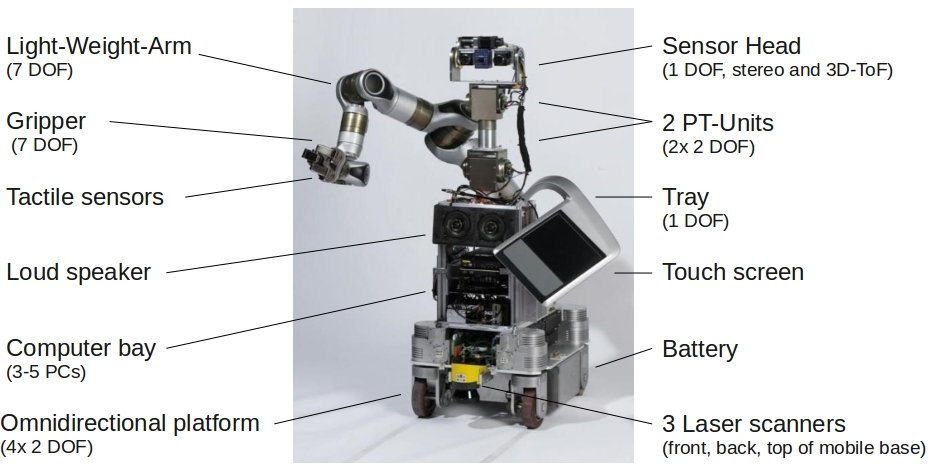
\includegraphics[width=\textwidth]{images/hw_setup_with_text}
\caption{Hardwarekomponenten des \cob}
\label{setup}
\end{figure}

  Die einzelnen Modelle unterscheiden sich aber in ihren
eingesetzten Komponenten. So ist der offensichtlichste Unterschied zwischen
den in Abbildung \ref{fig:vgl3336} abgebildeten cob3-3 und cob3-6 der von verschiedenen Herstellern stammende Arm. 

\begin{figure}[htb]
  \centering
  \subfigure[\cob3-3 mit \acs{LBR3}]{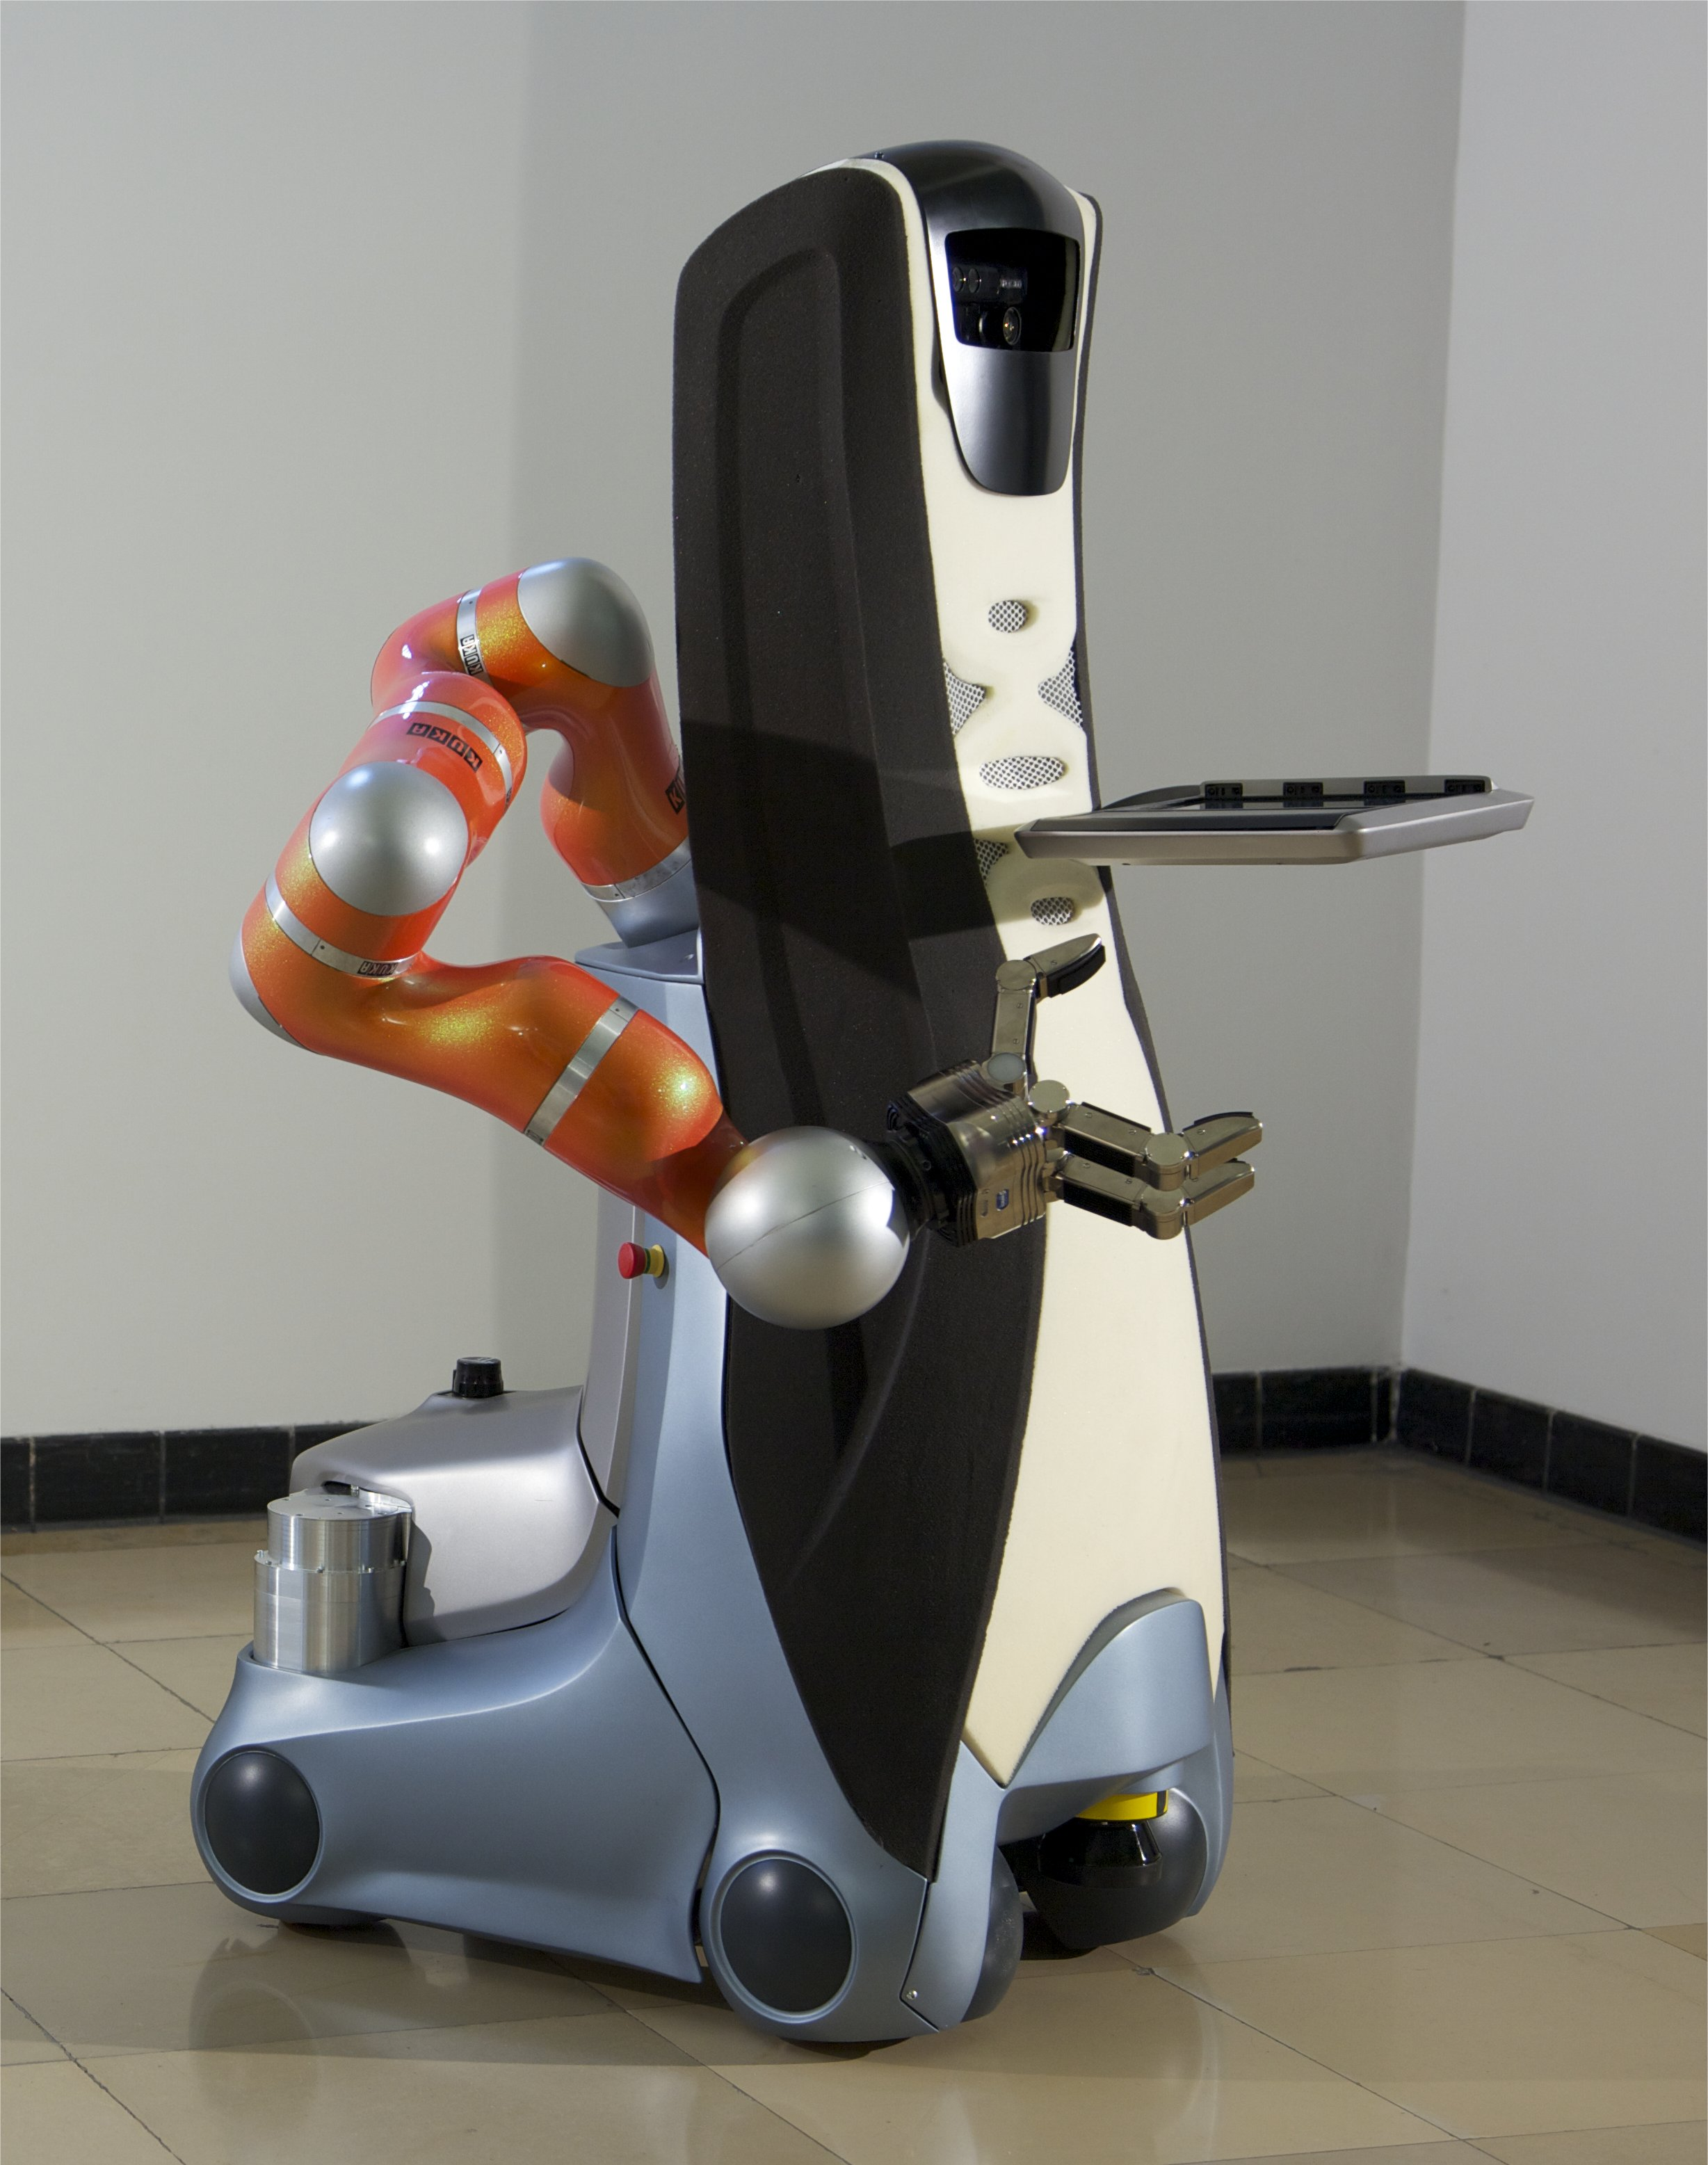
\includegraphics[width=.45\textwidth]{images/cob33lbr.jpg}}\hfill
  \subfigure[\cob3-6 mit \acs{LWA}]{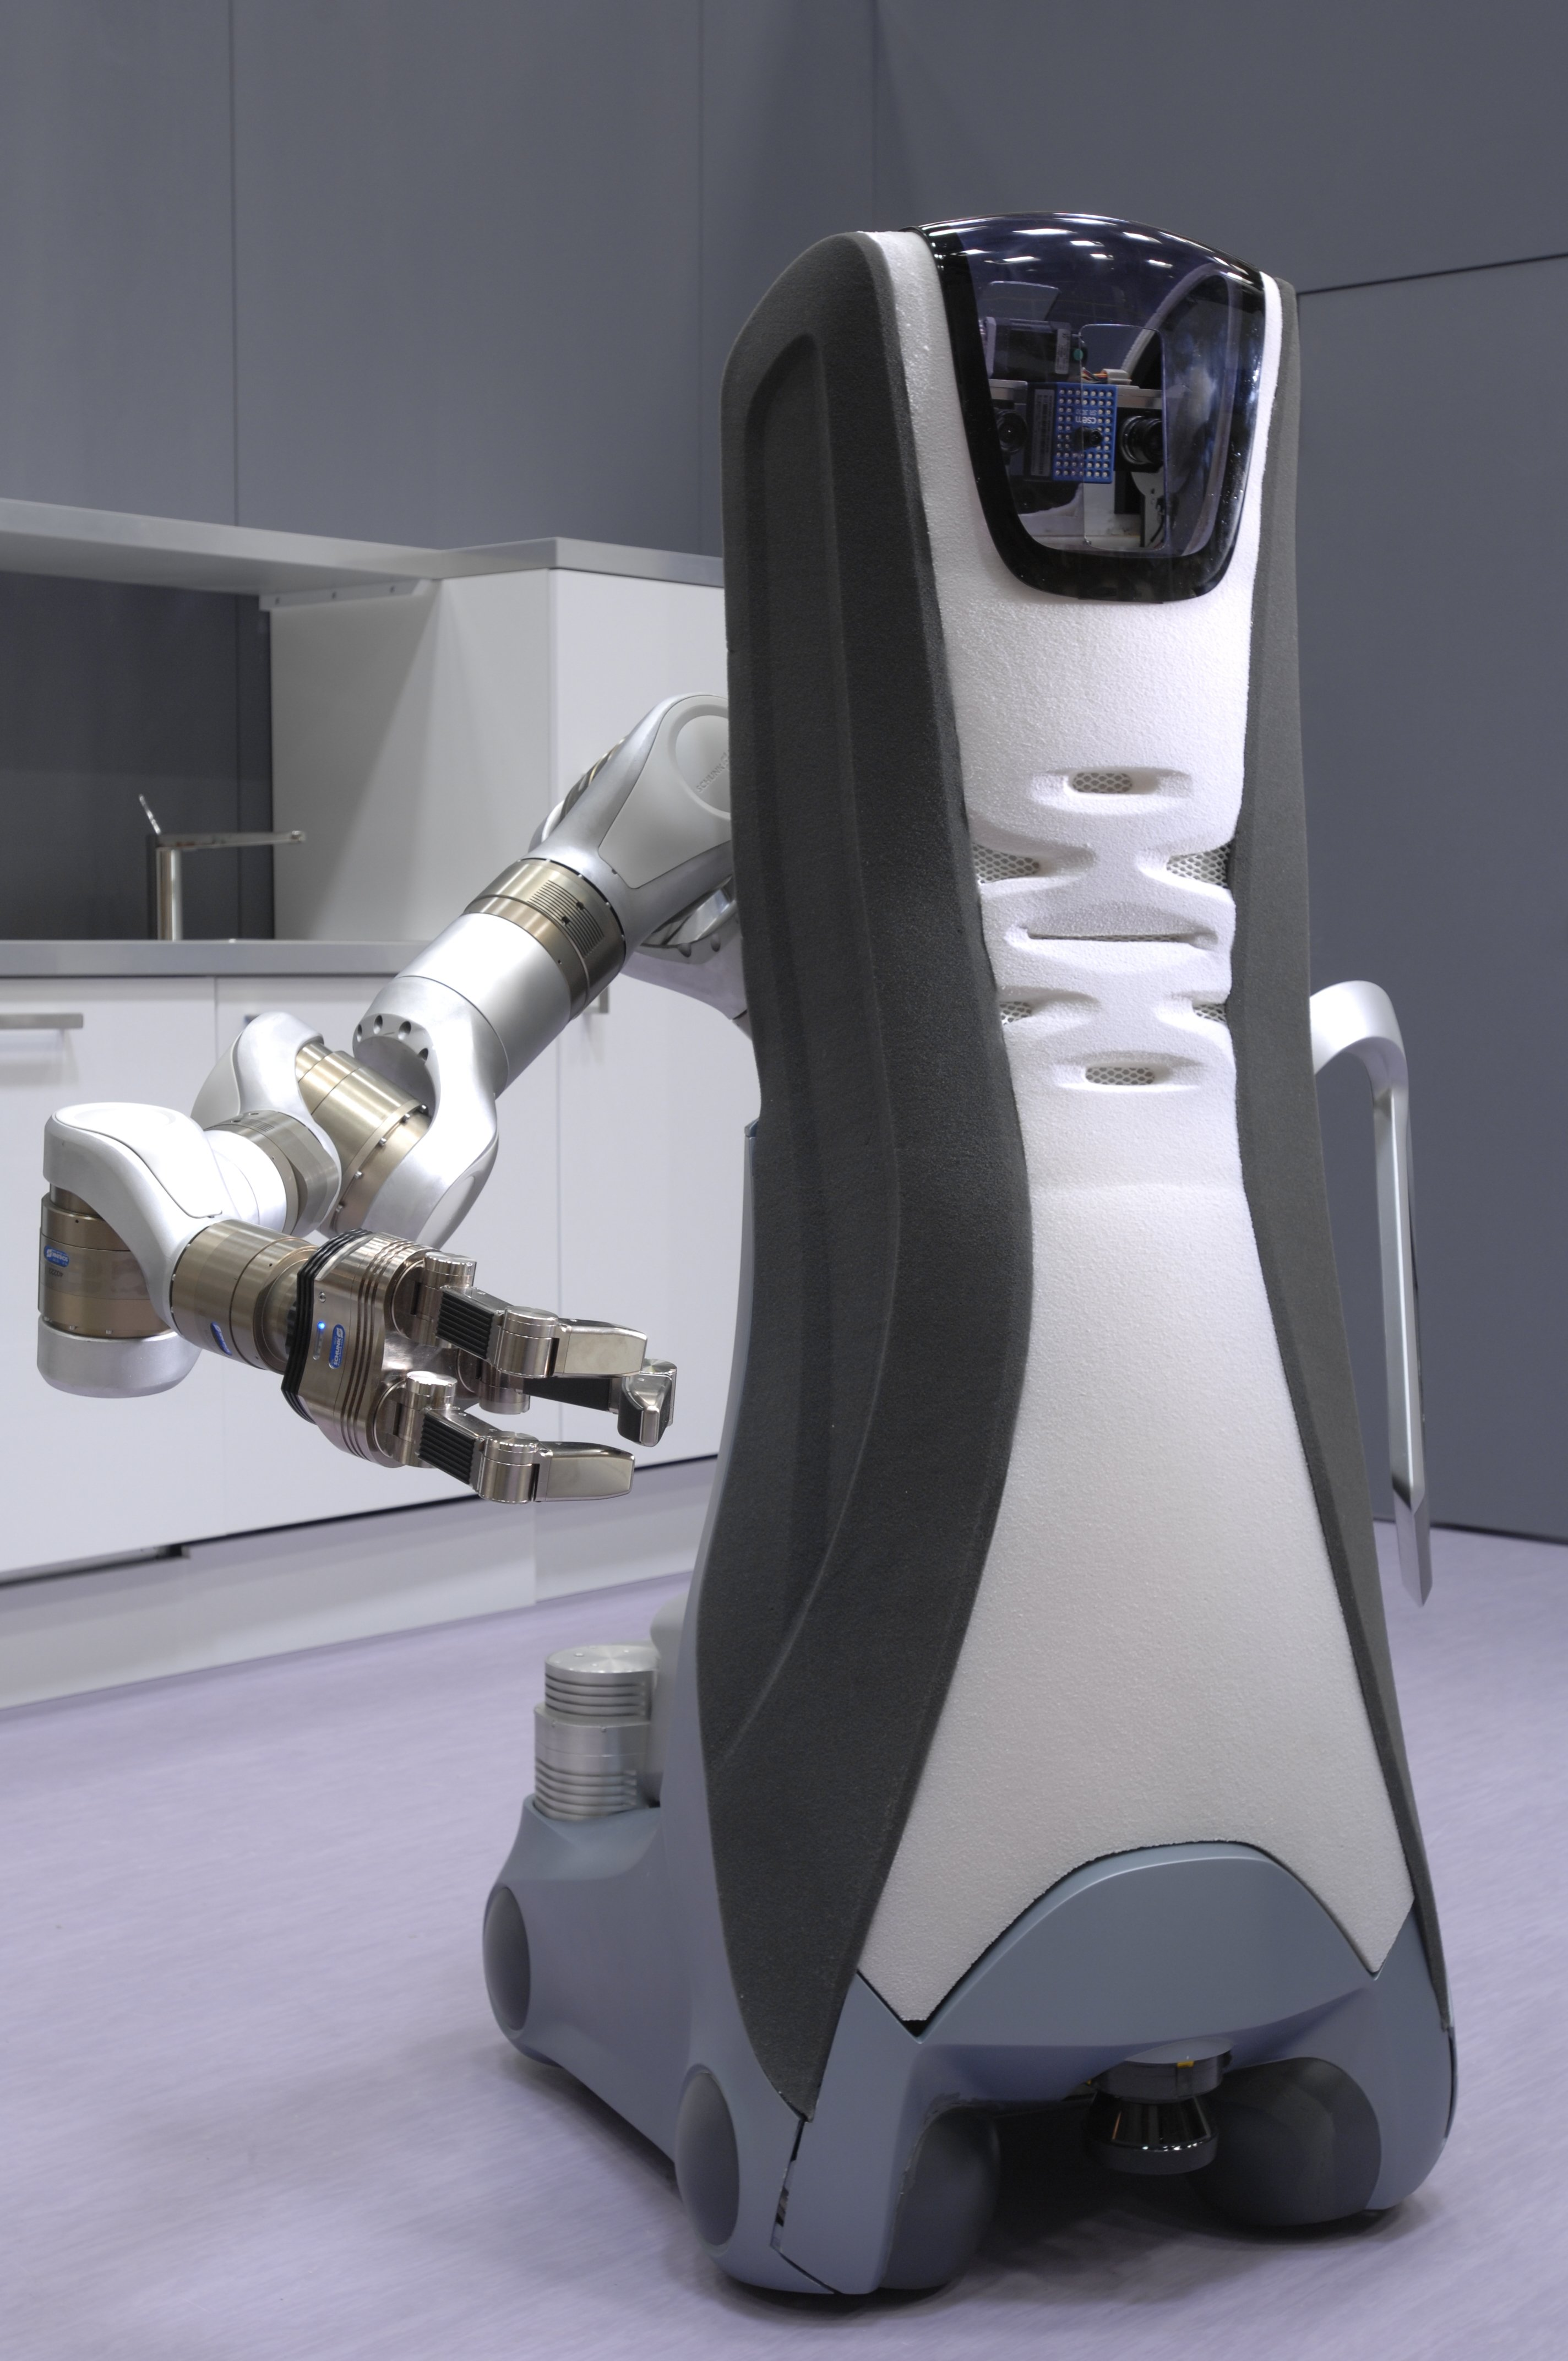
\includegraphics[width=.45\textwidth]{images/cob36lwa.jpg}}
  \caption{\cob3-3 und \cob3-6 im Vergleich}
  \label{fig:vgl3336}
\end{figure}

\subsection{Aktoren}

Die verschiedenen \cob Distributionen sind mit den folgenden Aktoren und Sensoren
ausgestattet, für die jeweils auch die Unterschiede zwischen den Modellen cob3-3 und
cob3-6 aufgelistet sind.

\begin{description}
  \item[Arm] Für den an der Rückseite des Roboters
    angebrachten Arm werden zwei Modelle eingesetzt. Einmal der \ac{LBR3} von
    Kuka sowie der \ac{LWA} von Schunk. 
  \item[Torso] Der Torso ist je nach
    Modellnummer ein 3 \ac{DOF} oder ein 4 \ac{DOF} Modell. Sowohl beim \cob
    3-3 als auch beim \cob 3-6 wird das 3 \ac{DOF} Modell eingesetzt.
  \item[Base] Als Basis für den Roboter dient eine omnidirektionale Plattform.
    Durch die vier in alle Richtungen lenkbaren Räder ist es dem Roboter möglich,
    aus dem Stand in alle Richtungen zu fahren oder zu drehen.
  \item[Tablett] Das Tablett kann beim \cob 3-3 hoch und runter geklappt werden
    und hat einen Touchscreen eingelassen, mit dem der Roboter bedient werden
    kann. Beim \cob 3-6 stehen mehr Freiheitsgrade zur Verfügung. Hier kann das
    Tablett zusätzlich entlang zwei Achsen gedreht werden. Dadurch kann die
    Bedienung vorallem für sitzende Personen bequemer gemacht werden. 
  \item[Hand]
    Als Hand wird die \ac{SDH} mit drei Fingern und sieben Freiheitsgraden
    eingesetzt. 
  \item[Kopfachse] Mit der Kopfachse kann die Kamera um \unit[180]{°} nach
    hinten geschwenkt werden, um sowohl im Manipulationsbereich hinter dem 
    Roboter als auch im Servicebereich vor dem Roboter Bildinformationen zu
    erhalten. 
  \item[Lautsprecher] Um dem
    Nutzer Rückmeldung über die aktuelle Tätigkeit des Roboters zu geben, sind in
    der Plattform Lautsprecher eingebaut.

\end{description}

\subsection{Sensoren}

\begin{description}
  \item[Kameras] Für die 3-dimensionale Bilderfassung werden
    verschiedene Systeme eingesetzt. Alle \cob der dritten Generation
    besitzen ein Stereokamerapaar aus zwei hochauflösenden Kameras.
    Darüber hinaus wird im \cob 3-3 eine Microsoft Kinect, im \cob 3-6 eine
    Asus X-Tion Pro und in anderen Modellen eine Time-of-flight Kamera
    eingesetzt. 
  \item[Laserscanner] Hinten auf der Plattform ist ein
    Laserscanner von Hokuyo verbaut, der für die Navigation eingesetzt wird.
    Außerdem ist vorne und hinten je ein Sicherheitslaserscanner von SICK
    verbaut, die zusätzlich den Not-Aus aktivieren, wenn sie ein Hindernis in
    unmittelbarer Nähe detektieren. 
  \item[Touchscreen] Zur Bedienung des
    Roboters ist im Tablett ein Touchscreen eingebaut. 
  \item[Taktile Sensoren]
    Damit der Roboter unterschiedliche Dinge sicher greifen kann, sind an der
    Hand taktile Sensoren angebracht, die die Greifkraft ermitteln können.
  \item[Mikrofon] Unter anderem zur Sprachsteuerung ist im Kopf des Roboters ein
    Mikrofon verbaut. Je nach 3D Kamera kann es auch in diese integriert sein.
\end{description}


%
% EOF
%

\section{Kalibrierungsbedarf} % (fold)
\label{sec:Kalibrierungsbedarf}
Wie jeder andere Roboter auch muss der \cob kalibriert werden. Durch Ungenauigkeiten bei 
der Montage oder Kollisionen beim Transport oder im Betrieb entspricht der Aufbau des \cob
nie dem auf der technischen Zeichnung. Obwohl diese Ungenauigkeiten selten größer als ein 
paar Millimeter oder Grad sind, können zum Beispiel Winkelfehler bei der Montage des Arms 
zu Abweichungen führen, die es dem unkalibrierten Roboter unmöglich machen, ein Objekt, dessen
genaue Position bekannt ist, zu greifen. Durch den Aufbau und Einsatz des \cob müssen 
Objekte erst von der Sensorik erkannt und im Raum lokalisiert werden. Wenn in diesem Schritt 
die Kameras an unbekannten Stellen des Roboters angebracht sind, kann aus den gewonnenen
Daten keine zielführende Aktion des Roboters berechnet werden. Ein erkanntes Objekt muss also 
erst im Kamerakoordinatensystem lokalisiert werden. Diese Position muss dann in ein zentrales 
Roboterkoordinatensystem umgerechnet werden. Teil dieser Transformation sind beim \cob mindestens
zwei unbekannte Einzeltransformationen. Dies ist die Montageposition des Torsos sowie die 
Position der Kameras auf dem drehbaren Kameraträger. Zusätzlich kann noch die Montageposition
des Kopfes auf dem Torso unbekannt sein. Ein Fehler an dieser Stelle kann aber auch durch die
zwei anderen Transformationen ausgeglichen werden. Um das Objekt schließlich greifen zu können,
muss die Position des Objekts relativ zum Ursprung des Arms bekannt sein, was eine genaue
Kenntnis der Montageposition des Arms vorraussetzt. Auf diesem Weg können sich kleine Fehler
zu großen Ungenauigkeiten beim Griff aufaddieren.

% section Kalibrierungsbedarf (end)
